\subsection*{Acquired predictions alter actual maintenance, with a limited return under equal purchases}

The birth/death material CA allows a physical question that the conservative action tests cannot answer: can acquired experience change how a body protects tissue that is continually being produced and lost? We equip the externally supplied density-regulated host with a local protective reserve. Two initially neutral warning labels precede weak or strong mechanical contact. A standard conditional delta rule updates from the incident mechanical strain actually sensed during contact, including contact absorbed by protection. It does not receive a future damage field or the hidden label--strain relationship. The sensor thus measures an actual but relatively informative physical variable. Protection purchased from real precursor and old tissue energy is present before contact, absorbs demand and is depleted or lost with tissue (Fig.~\ref{fig:predictive-maintenance}).

Initial comparisons retain uniform, instantaneous and full fixed protection as well as the standard mean predictor and a higher-capacity risk predictor. The risk predictor's limited damage reduction accompanies additional protection and memory expense; no extra predictor advantage is established. Full fixed protection gives the lowest absolute loss with greater sustained investment. A later content test preserves the learned quantities and changes their readout: use the correct conditional content, pool the two labels, or exchange them. An initial attempted uniform-purchase match is limited by local capacity and payment, so it is not called equal purchasing. The actual equal-purchase test instead supplies a fixed common per-step quota that every branch realizes to floating-point precision.

From two complete acquired parents, correct conditional content reduces 96-step tissue injury from $5.43517$ to $4.53509$ and from $7.10679$ to $6.74210$ relative to pooled content, approximately 16.6\% and 5.1\%. Swapping content raises injury to $6.69137$ and $7.71390$. Correct content leaves more tissue and slightly more subsequent uptake in both parents. Its first terminal energy, however, is $90.61563$ versus $90.73901$ under pooling. Equal purchased protection and synthesis price do not equalize reserve holding, memory, movement or birth costs as bodies diverge. These finite comparisons show that already acquired conditional content can guide a useful physical allocation; they do not establish a new predictor, exclusive newborn plasticity or a general net benefit (Supplementary Table~\ref{tab:maintenance-equal}).

\subsection*{Stronger physiology limits the benefit attributed to predictive maintenance}

We next restore the same two acquired parents and compare six policies under the same purchase allocator: continued delta learning, frozen learned content, each of two fixed label mappings, an immediate response to completed strain, and uniform allocation. Both fixed mappings are run unchanged in both worlds; we do not select the better mapping after seeing the hidden relation. The first 96 steps preserve that relation, then 96 steps introduce an unannounced change. Continued learning reduces post-change injury relative to frozen content by 9.17\% and 10.24\%. Nevertheless, it loses 7.51\% and 4.83\% more tissue than the immediate physiological response. Uptake, energy and mass provide no uniform post-change dominance over that response or uniform allocation. Improving over obsolete frozen content therefore does not establish that continued prediction is generally better than responsive physiology.

For readout comparison, all six policies carry and pay for the same four predictor/eligibility scalars, although fixed, instantaneous and uniform controls do not need all of them. This extra capacity charge makes those controls conservative economic comparators, not their cheapest possible implementations. Actual purchases are matched, but total expense remains state-dependent. The corresponding full 192-step injury advantage of delta over the immediate response is only about 1.27\% and 0.22\%, with opposing uptake and terminal-energy trade-offs. We retain all twelve paths and all three reporting windows (Supplementary Tables~\ref{tab:maintenance-strong} and \ref{tab:maintenance-costs}).

The registered tissue cohort supplies a second physical check. Tissue present at the complete parent is labelled before branching, and its actual removal by contact, starvation and rule death is tracked through material transport. Birth does not add to this old cohort. The strong-control futures retain about 70.5--75.4 units of later-born tissue while accumulating about 130.6--133.9 units of birth. These are different stocks and flows; neither high turnover nor continued protection identifies a causal requirement for correctly copied newborn content. The earlier newborn zero/swap outcomes remain relevant negative controls.

\subsection*{Contact timing changes the value of prepared reserves within a stable relationship}

A prospective timing intervention holds the learned warning relationship fixed. Two actual intermediate parents each supply four 96-step futures: frozen learned readout or immediate physiology, with a four-step distributed contact or its externally integrated strain concentrated into the first step. Warning, contact onset and interval remain matched. Predictive writing is disabled throughout, excluding different numbers of within-contact learning updates as the explanation. Bodies and later physical feedback can nevertheless diverge, so the intervention does not isolate event-time replenishment as a unique mediator.

Relative to immediate physiology, the learned readout reduces injury by 5.42\%/6.51\% for distributed contacts and 8.69\%/5.98\% for concentrated contacts. Uptake, final mass and final energy are slightly higher in all four conditions. Concentrating contact increases the absolute injury difference by $0.27094$ and $0.02758$ in the two parents; the second effect is small, and proportional benefit does not rise in both. These are finite benefits of ordinary delta-acquired content under a preserved relation, not successful learning of the previously changed relation (Supplementary Table~\ref{tab:maintenance-timing}).

The physical distinction is informative. If every site had the same constant marginal avoidable loss $\beta$ and a common maintenance budget $B$ could always be usefully spent, total prevention would be $\beta B$, regardless of prediction accuracy. Here actual prevention is the sum of $\min(\text{reserve},\text{demand})$ over local contacts. Saturation, reserve decay, tissue loss and local capacity restrict when and where a purchase remains useful. The observations show a setting in which allocation and timing can matter, while the strong controls reveal how modest and conditional the realized benefit is. They do not partition all these physical causes or supply evidence for the uncompleted successor mechanism. The conservative learner and the regenerative maintenance body remain distinct experimental systems.

\begin{figure}[p]
\centering
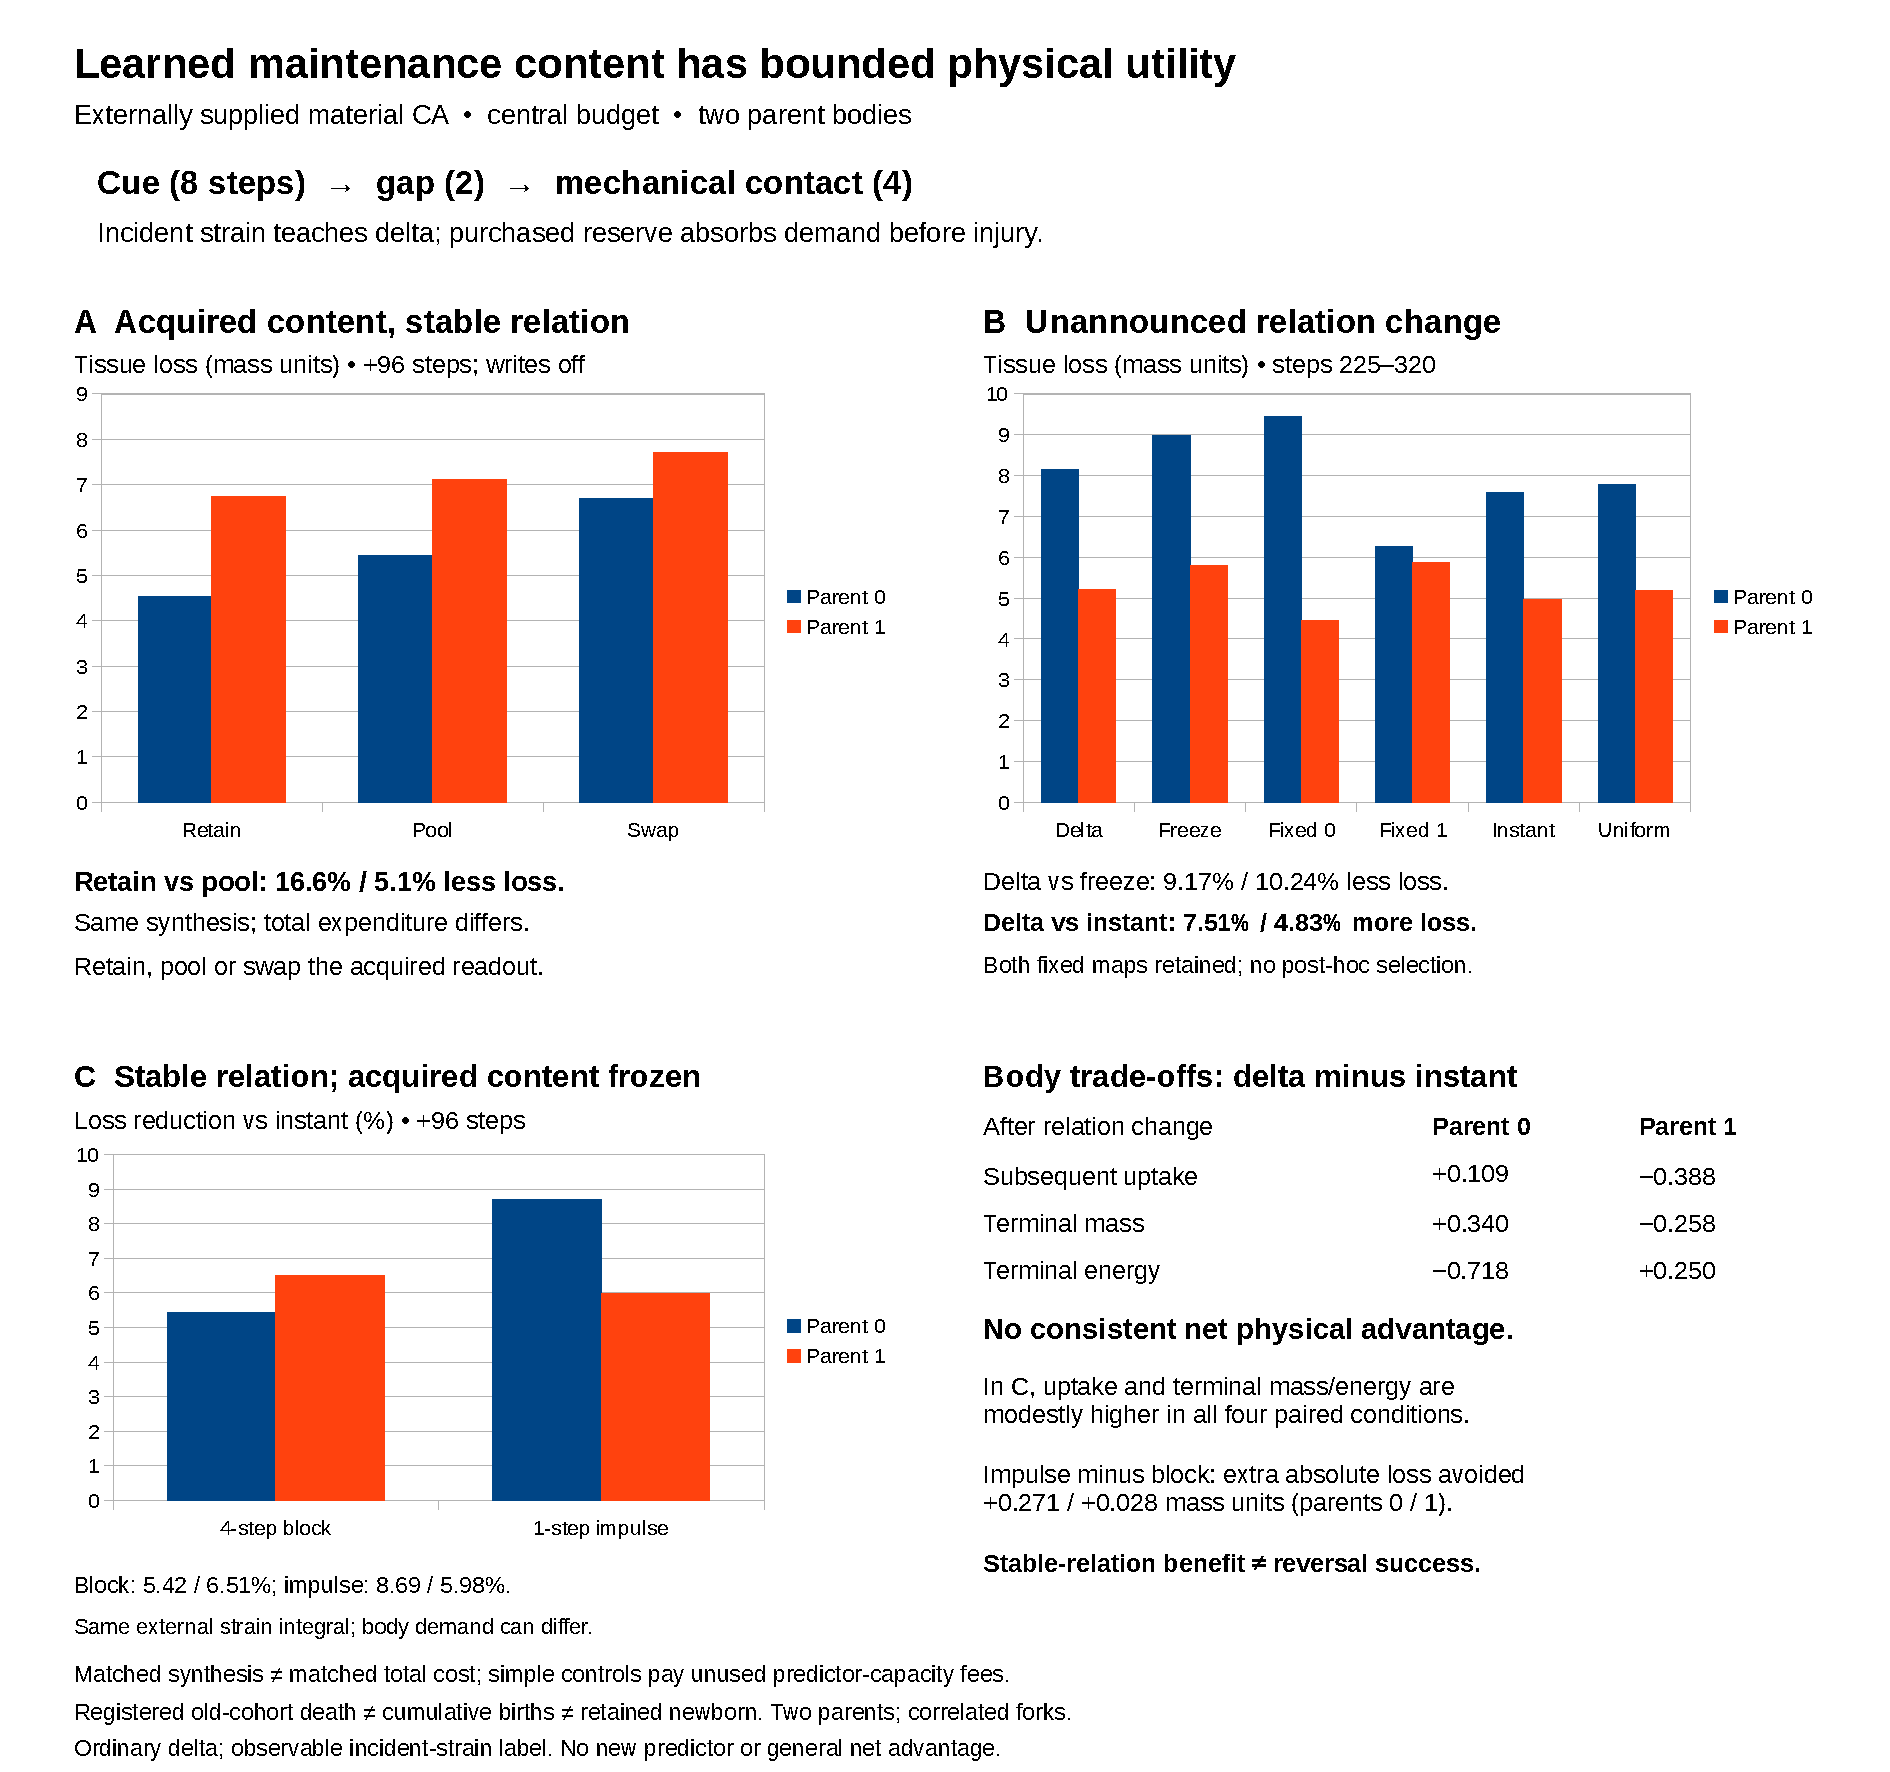
\includegraphics[width=\linewidth,height=0.63\textheight,keepaspectratio]{work/longform_v047/figures/predictive_maintenance_v048/predictive_maintenance.pdf}
\captionsetup{font=footnotesize}
\caption{\textbf{Acquired conditional maintenance has limited physical utility against strong instantaneous controls.}
The externally supplied, density-regulated material CA has centrally coordinated purchasing and a local incident-strain sensor. The ordinary conditional delta rule learns from completed contact, including strain absorbed by reserve; it is not a new predictor.
\textbf{a}, All three content readouts of two acquired parents over 96 new steps with writes stopped and the learned relation retained. Retaining rather than pooling content reduces injury by 16.6\%/5.1\% at equal realized reserve synthesis; swapping also raises injury.
\textbf{b}, All six policies from both actual parents. Bars show injury in steps 225--320 after the relation changes at boundary 224. Continued delta reduces injury relative to frozen content by 9.17\%/10.24\%, but loses 7.51\%/4.83\% more tissue than the instantaneous rule. Neither fixed map is selected retrospectively. The accompanying delta-minus-instantaneous contrasts show opposed uptake and terminal mass/energy effects, without consistent net benefit.
\textbf{c}, Two actual 192-step parents each supply four 96-step futures under the retained relation, crossing block/impulse contact with acquired/instantaneous readout; writes are frozen. External strain integrals match, while realized bodily demand can differ. Bars show paired injury reductions relative to instantaneous allocation. The impulse increases the absolute avoided-loss contrast by 0.271/0.028 mass units, but proportional benefit does not rise in both parents. This is a stable-relation expression test, not reversal success or isolation of one timing mediator.
Colours identify source parents within each assay; their branches are correlated conditions. Equal synthesis does not equalize total expenditure. Simple controls carry unused predictor capacity and its fees. Old-cohort death, cumulative birth and retained newborn tissue are distinct; none establishes newborn-content necessity. The original missing risk tail is not imputed. Full phase outcomes and physical accounts are in the accompanying maintenance source tables.}
\label{fig:predictive-maintenance}
\end{figure}

